% !TeX encoding = UTF-8
% !TeX spellcheck = en_US
% !TeX root = ../../Thesis.tex

\chapter{Cathodic Ray Tube Basics}

This section features a quick explanation what a CRT is and what it's main components are, followed by a more detailed description on how these components are implemented in the CRT Heerlen D14-363GY, which was used in this project. It ends with a description of the important characteristics of the CRT and the requirement the theory poses on them.

\section{Underlying Physics}

Wikipedia states: ``The cathode-ray tube (CRT) is a vacuum tube that contains one or more electron guns and a phosphorescent screen and is used to display images. It modulates, accelerates, and deflects electron beam(s) onto the screen to create the images.''

There are three vital components to accomplish this feat: the electron gun, the electron lens and the deflection plates.

\begin{figure}
	\centering
	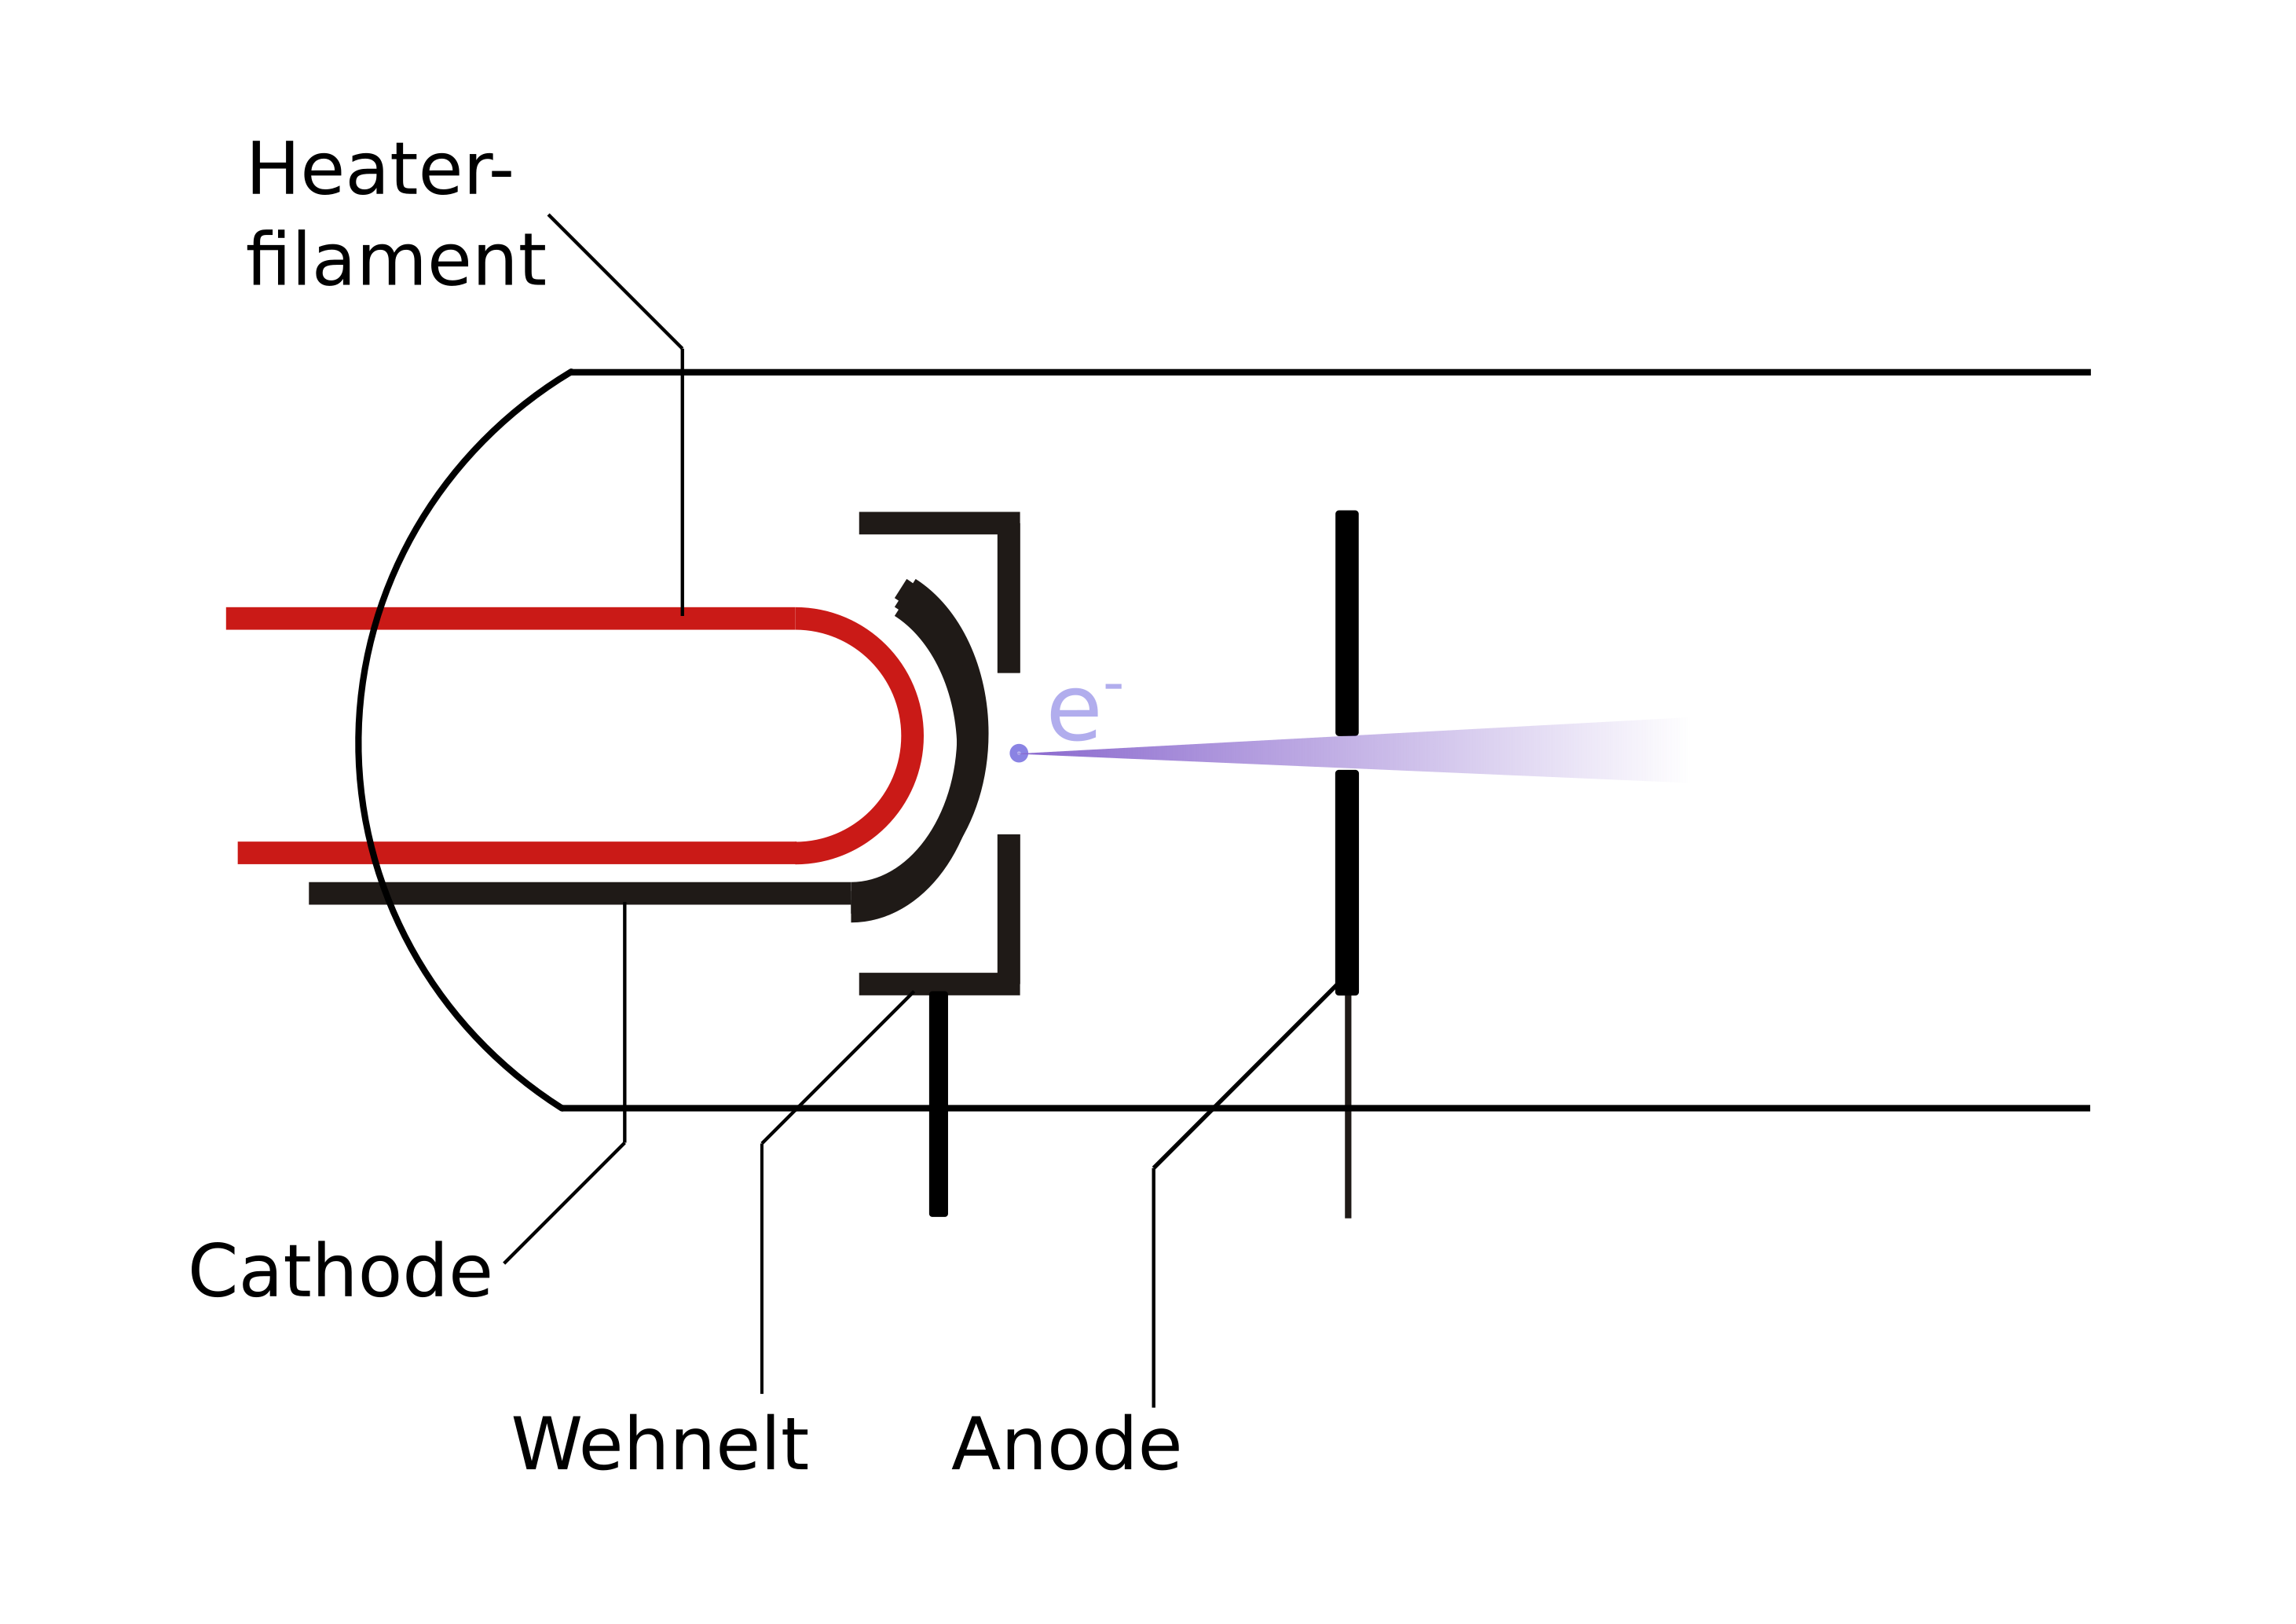
\includegraphics[width=0.7\textwidth]{Chapters/CRT-Basics/electron_gun}
	\caption{Schematic of an electron gun}
	\label{fig:electrongun}
\end{figure}


The electron gun extracts electrons from a cathode material, accelerates them onto a perforated anode and thereby produces a free electron beam (see \cref{fig:electrongun}). One important characteristic in the selection of a cathode material is a low work function. The work function denotes the amount of energy needed to extract one electron from the material. The are two ways to overcome this energy barrier in an electron gun, one can either overcompensate it by applying a strong electric field (``field emission'', ``cold cathode'', \cref{fig:hotcathodecoldcathode} b) or one can heat the material until some electrons have enough thermal energy to overcome the energy barrier (``thermal emission'', ``hot cathode'', \cref{fig:hotcathodecoldcathode} a). For our CRT, only thermal emission is relevant, more detail on this will be added later along with the description of our cathode's design. 

\begin{figure}
	\centering
	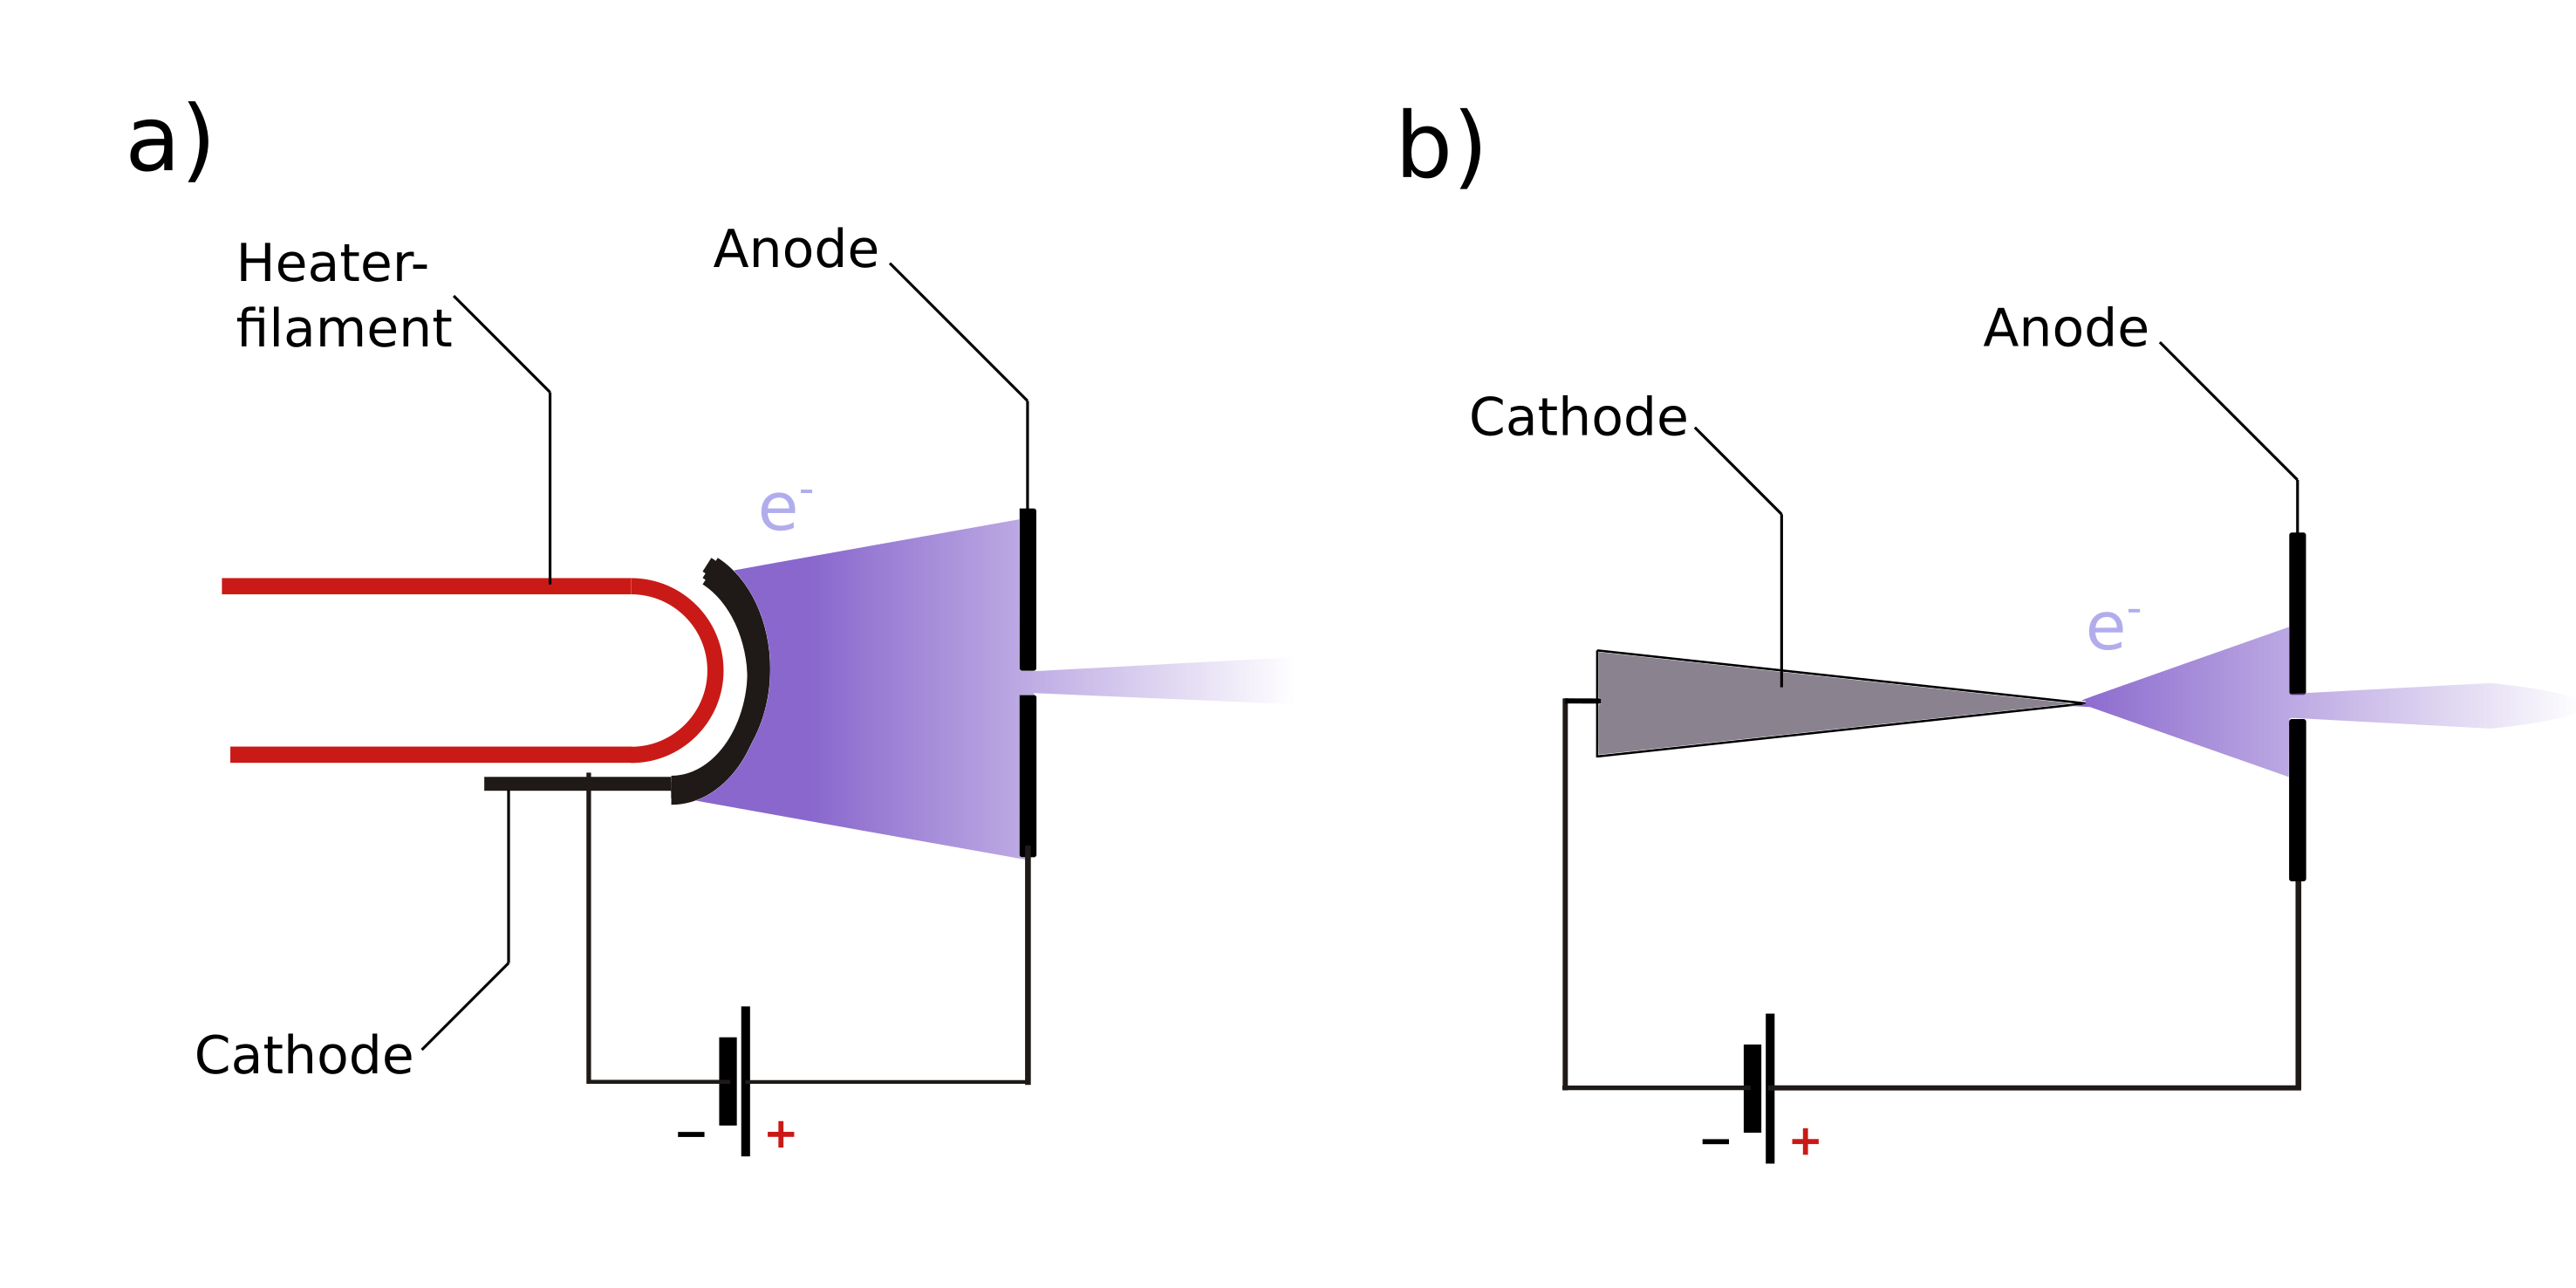
\includegraphics[width=0.9\textwidth]{Chapters/CRT-Basics/HotCathodeColdCathode}
	\caption{a. Schematic of a hot cathode; b. Schematic of field emission cathode}
	\label{fig:hotcathodecoldcathode}
\end{figure}

The cathode itself is housed in a so-called Wehnelt cylinder, as the name suggests it is conducting cylinder, which is set to a slightly more negative potential than the cathode itself. This part implements two features, firstly it condenses the emitted electrons, leading to a smaller spot size, i.e. making the cathode a more point-like electron source. Secondly it enables us to regulate the beam current, the more negative the Wehnelt potential is, the less electrons are emitted by the electron gun. As we make the Wehnelt potential more positive, the beam current increases and continues to rise even after it is more positive than the cathode itself. However the spot size reduction is lost in the process, along with the ability to properly focus the beam with electron optics.

The electrons that leave the electron gun are still divergent and need to be focused. For our \SI{2}{\kilo\electronvolt} electrons it is still possible to use an electrostatic lens. Cylindrically symmetrical pieces of conductor, like rings and tubes, can be set to an electrical potential and act as a lens for the electrons. By combining several of them, one can (theoretically) engineer an electro-optical system with any combination of desired focal lengths $f_1$ and $f_2$. The field of this system is simply governed by Laplace's equation in cylindrical coordinates:
\begin{equation}
	0=\dfrac{1}{r}\pdv{\phi}{r}+\pdv[2]{\phi}{r}+\pdv[2]{\phi}{z}
\end{equation}
If we take the axis of the beam to be the z-axis, the position of the focal point in the x-y-plane can be shifted using the two pairs of deflection plates, one for the x- and one for the y-direction. The deflection is achieved by applying a voltage between the two parallel plates. (see: \cref{fig:deflectionplate2}) By starting with an electron with kinetic energy $e \cdot U_0$ which is accelerated in x-direction by a constant force $e\cdot U_x / d$ over the extent of the plates $L$, the deflection angle is approximately \cite{Demtroeder3}:
\begin{equation}\label{key}
	\delta \approx \tan(\delta) \approx \frac{U_x\cdot L}{2 U_0 \cdot d}
\end{equation}

For the measures of our CRT ($ L \approx \SI{10}{\centi\meter}$, $d \approx \SI{1}{\centi\meter}$, $U_0 \approx \SI{2}{\kilo\volt}$ and distance to screen $\approx \SI{20}{\centi\meter}$) this amounts to a deflection coefficient of around \SI{20}{\volt\per\centi\meter}, which is quite consistent with the value given in the CRT's manual.\todo[]{können die Maße stimmen?} 

\begin{figure}
	\centering
	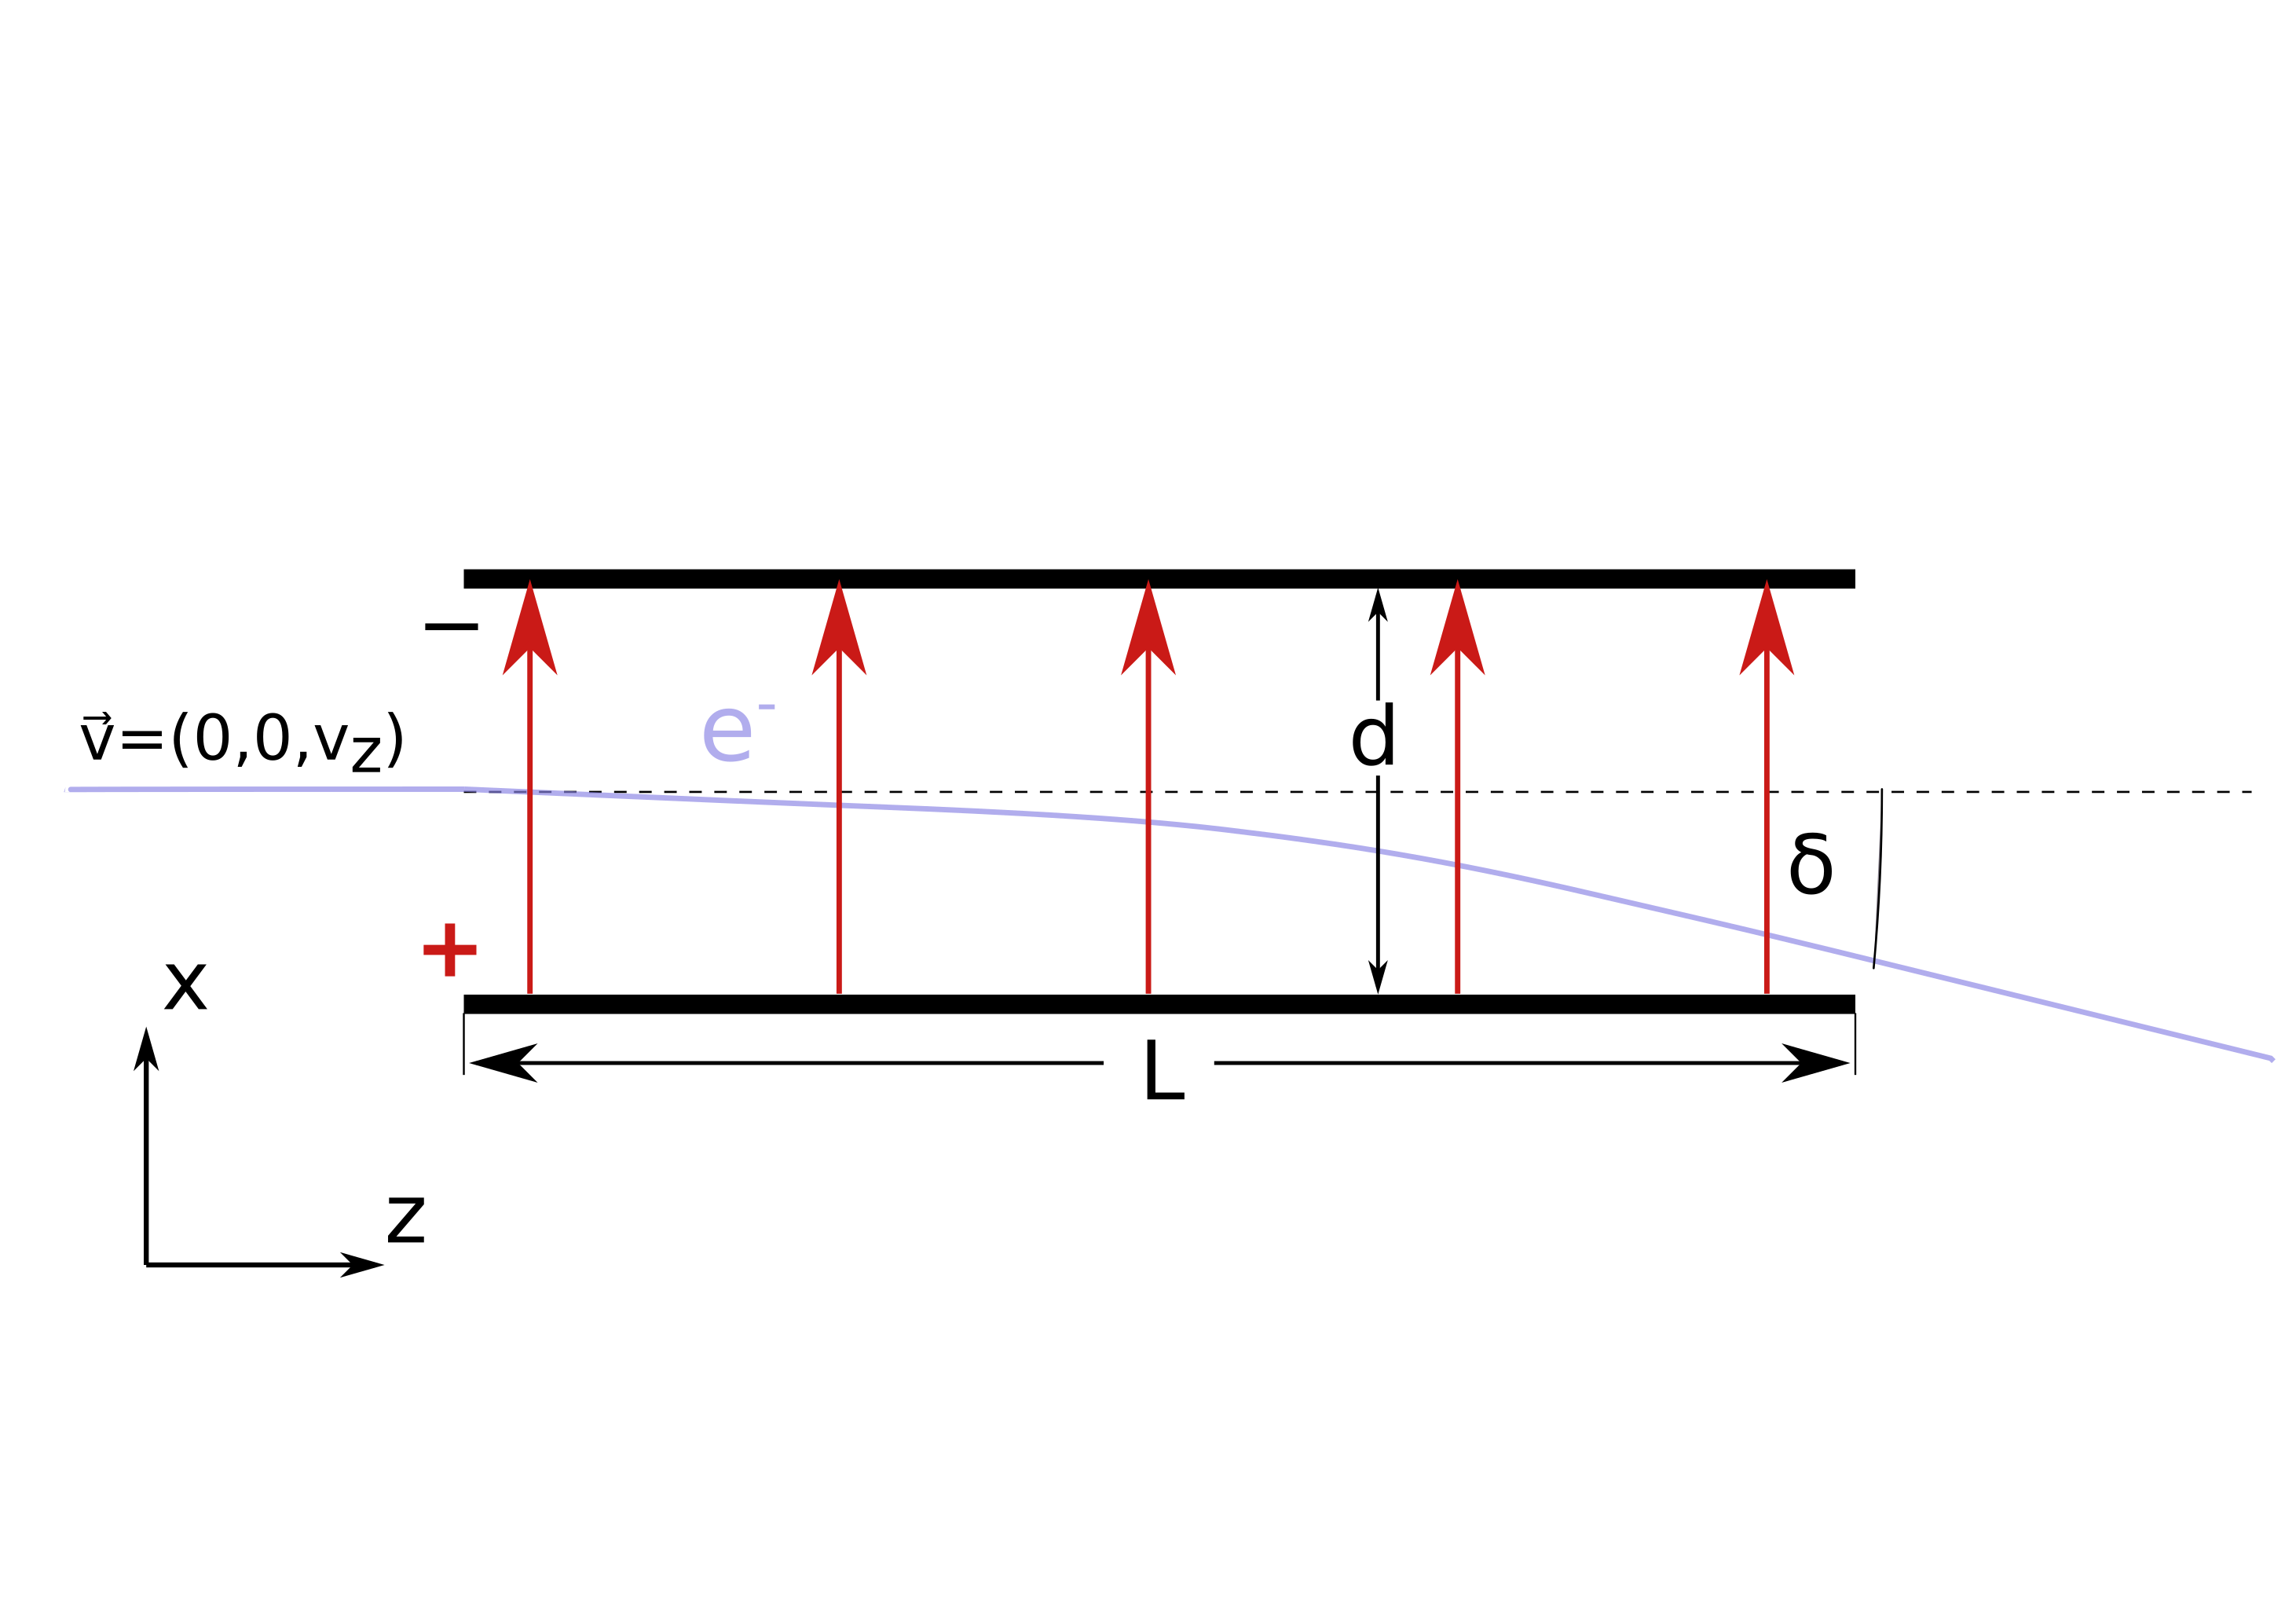
\includegraphics[width=0.7\textwidth]{Chapters/CRT-Basics/DeflectionPlate2}
	\caption{Deflection of an electron beam in a constant electrical field}
	\label{fig:deflectionplate2}
\end{figure}

\section{Implementation in the Heerlen D14-363GY }

This section describes how the mechanisms described above are implemented in the CRT that was used in this project: the PDS/CRT Heerlen D14-363GY. \Cref{fig:FotoCRT} shows an image of said CRT, \cref{fig:SchemeCRT} shows a schematic depiction. The cathode is not visible, as it is fixed inside the Wehnelt cylinder (1), just a few millimeters from the exit of the wehnelt cylinder the electrons pass through the perforated anode (2) they gain their full final kinetic energy over this short distance. The electrons that go through the perforation and enter the electrostatic lens, have \SI{2}{\kilo\electronvolt} and therefore move at a speed of approximately \SI{0.08}{\clight}. 
The electrostatic lenses are realized using three conducting rings (3), that are set to the same potential but have varying radii: Each consectutive ring has a smaller radius than the previous one. 

\begin{figure}
	\centering
	\begin{subfigure}{.5\textwidth}
		\centering
		\missingfigure[figwidth=0.9\textwidth]{Image of CRT}
		%\includegraphics[width=.9\textwidth]{"".png}
		\caption{Image picture of the Heerlen D14-363GY}
		\label{fig:FotoCRT}
	\end{subfigure}%
	\begin{subfigure}{.5\textwidth}
		\centering
		\includegraphics[width=.9\textwidth]{"Chapters/CRT-Basics/electrode configuration".png}
		\caption{Schematic of the CRT from \cite{D14363GY123-manual}}
		\label{fig:SchemeCRT}
	\end{subfigure}
	\caption{}
	\label{}
\end{figure}


Between the electrostatic lens and the deflection plates, there is another aperture (4), which is internally connected to the anode and is thereby kept at the same potential. In our Setup, the deflection plates are not simply parallel but are shaped like funnels (5,7), between the two pairs of deflection plates, we have the final aperture (6), this ones potential can be regulated separately (usually it's on the same potential as the anode) 

It is connected to the glass envelope of the CRT to prevent the glass from charging up and distorting the image. 
Finally the beam hits the phosphorous-coated screen which fluoresces on electron impact.

\subsection{The Cathode}

As already mentioned, we are using a hot cathode, where the electrons are exited thermally until some of them acquire enough energy to leave the material. Compared to cold cathodes, which work by field emission, this leads to a broader energy distribution. In fields like electron microscopy, where a high resolution is the goal, this in undesirable, as it leads to some degree of chromatic aberration in the electron optics, for our purposes, this should not be a problem. On the other hand, hot cathodes normally allow for higher current densities, which is very important to us. The  electron current from this kind of emission is described by \cite[chp 3.2.3]{Whitaker}: 

\begin{equation}\label{eq:thermionic_current}
I=A\cdot T^2 \cdot e^{-b/T}
\end{equation}

Where $b$ is proportional to the the work function of the material, $T$ is temperature and $A$ is a material-dependent constant. It is clear from this formula, that a low work function and a high melting point are important characteristics for a good cathode material. 

The cathode from one of our Heerlen D14-363GY-tubes has been removed and examined with EDX (Energy-dispersive X-ray Spectroscopy). Nickel, barium, and strontium have been found, which suggests that it is a metal oxide cathode with barium-, strontium-, and possibly aluminum-oxide. This type of cathode is very common in low power electron tubes.

%add figure \todo{insert SEM image}

The ``Power Vacuum Tubes Handbook'' \cite[chp 3.5.2.1]{Whitaker} describes a typical oxide cathode as a coating of barium and strontium oxides on a structure made from nickel alloys. Nickel is chosen for it's strength and toughness, which it retains even at high temperatures. These cathodes are normally made by coating a case structure with a mixture of barium and strontium carbonates (typically \SI{60}{\percent} Ba and \SI{40}{\percent} Sr), suspended in a binder material and then baking the structure, causing the carbonates to be reduced to oxides.

These metal oxide cathodes normally operate at \SIrange{700}{820}{\celsius} and are capable of average emission densities of \SIrange{100}{500}{\milli\ampere\per\centi\meter\squared}. Still higher peak emissions are possible for shorter periods of time, as already mentioned, one of the advantages of this type of cathode is its high emission current capability compared to cathodes made from other materials. Downsides to this cathode type are its greater susceptibility to so-called oxygen poisoning and to ion bombardment. The literature therefore recommends to avoid prolonged exposure to oxygen. Oxygen poisoning is the process in which oxygen adsorbs onto the cathode and increases its work function, effectively reducing its ability to emit electrons. 
Also the material from the oxide cathode will evaporate during the tube's lifetime and will travel to other parts of the tube, adsorbing to electron optics parts and turning them into additional emitters. The literature (also from \cite{PowerTubes323Avadhanulu}) therefore also advises against exceeding the design value for the heater voltage, as this reduces the lifetime of the cathode significantly. (However during the course of our project, we did drive the cathode with higher heater voltages on various occasions in order to increase the available beam current.)

\subsection{Cathode Layout}

\Cref{fig:cathodelayout} shows how metal oxide cathodes for CRTs typically look, the depiction agrees very well with the layout of our cathode. On the image we see the cathode cylinder, which corresponds to the nickel support structure mentioned above. It is shaped into a cup, i.e. the cylinder is hollow and open on one side, where the heater filament (shaped into a heater coil) is inserted. The oxide disk, from where the electrons are emitted, is baked onto the top of the cathode cylinder. The cathode cylinder is mounted on an isolating support structure and inserted into the Wehnelt cylinder, which is called ``grid cup'' in the drawing. 
  

\begin{figure}
	\centering
	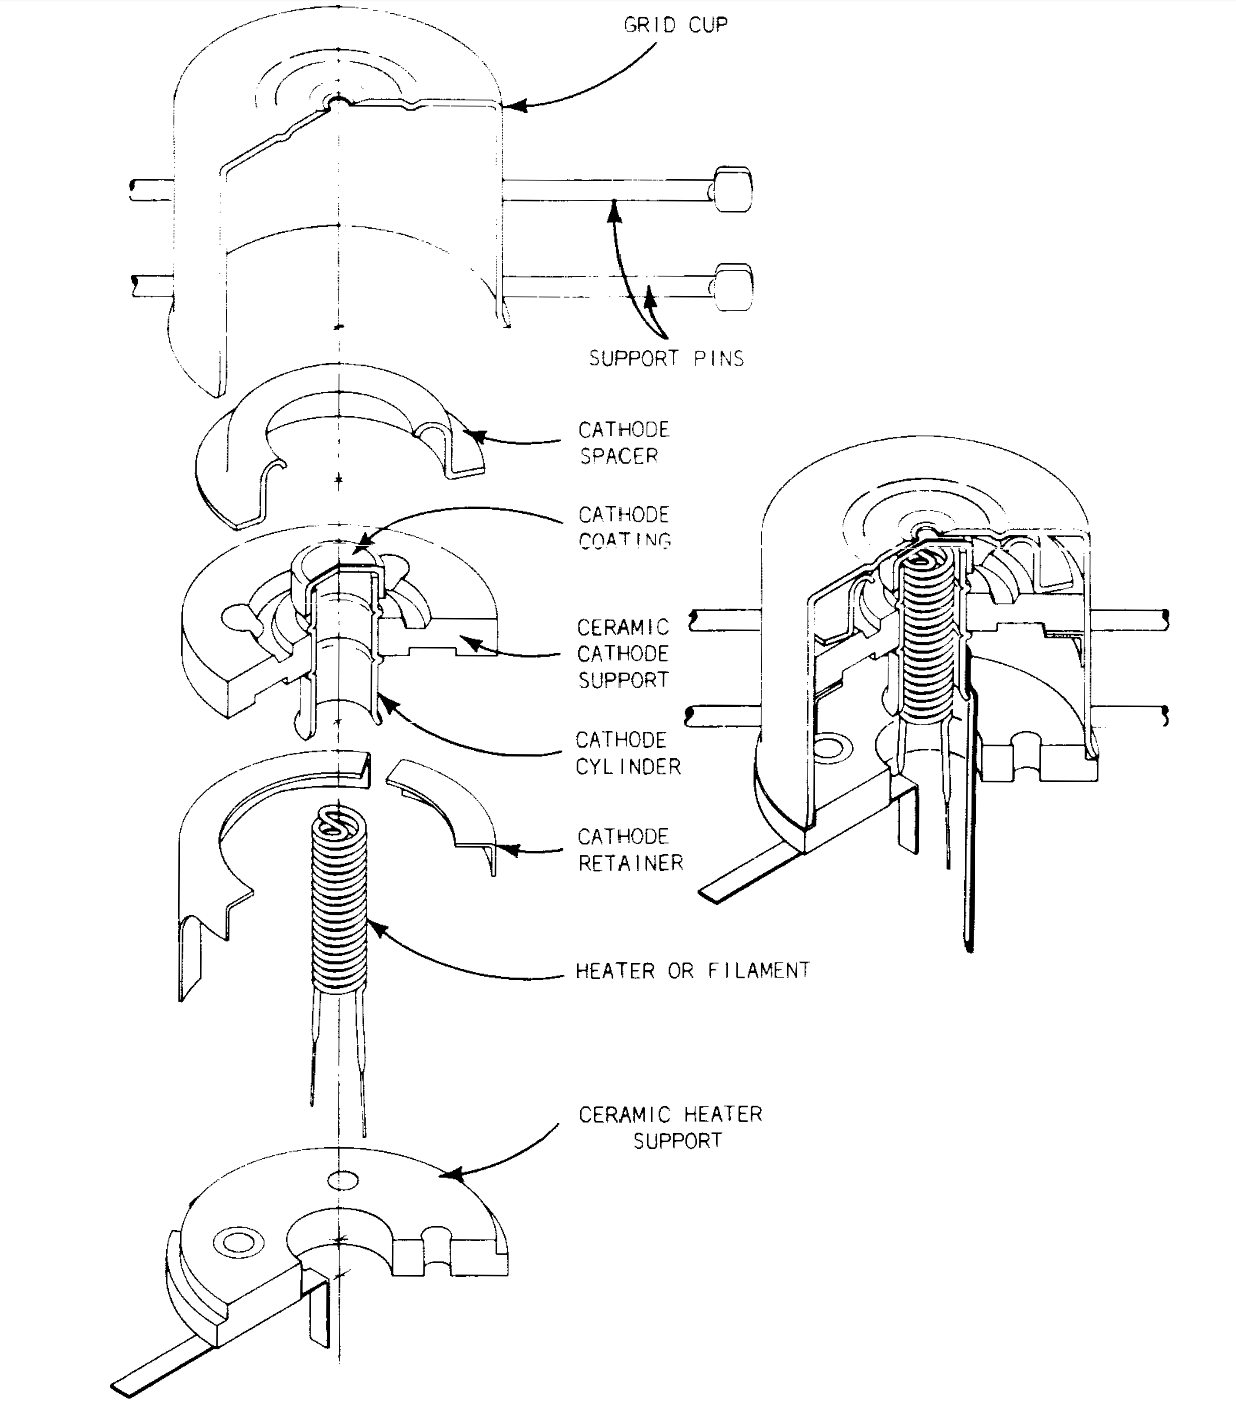
\includegraphics[width=0.6\textwidth]{Chapters/CRT-Basics/Cathode_layout}
	\caption{Schematic of the layout of a typical CRT-cathode from \cite{deVere69}}
	\label{fig:cathodelayout}
\end{figure}














